
\documentclass[a4paper, 12pt]{article}
\usepackage{geometry}
\geometry{margin=2cm}
\usepackage{graphicx} % Required for the inclusion of images
\usepackage[utf8]{inputenc}
%\usepackage{natbib} % Required to change bibliography style to APA
\usepackage{amsmath} % Required for some math elements 
\usepackage[spanish]{babel} 
%\usepackage{fontspec}
\usepackage{lineno,hyperref}
\usepackage{upgreek}
\usepackage{gensymb}
\usepackage{textcomp}
\usepackage{amssymb}
\usepackage{textgreek}
\usepackage{float}
\usepackage{fancyhdr}
\usepackage{dirtytalk}

\allowdisplaybreaks
%\textwidth18cm
%\textheight22cm
%\topmargin0cm
%\oddsidemargin2cm
%\hypersetup{hidelinks}

\usepackage{multirow}

\hypersetup{
    colorlinks=true,
    linkcolor=blue,
    }
\graphicspath{{img}}
\setlength\parindent{0pt} % Removes all indentation from paragraphs

\renewcommand{\labelenumi}{\alph{enumi}.} % Make numbering in the enumerate environment by letter rather than number (e.g. section 6)

\renewcommand{\b}{\textbf}

\newsavebox{\mygraphic}
\sbox{\mygraphic}{
\includegraphics[height=1cm]{logoUNRN.jpg}}


\pagestyle{fancy}

\fancyhead{}

\headheight 16pt

\fancyhead[LO]{\setlength{\unitlength}{1in}
	\begin{picture}(0,0)
		\put(0,0){\usebox{\mygraphic}}
	\end{picture}
	\hspace{1cm}
}

\fancyhead[CO] {\hspace{1.5cm} \large Física I: Ingenierías Ambiental, Electrónica y Telecomunicaciones}

%esto me pareció piola para enumerar los ejercicios
%lo saqué de acá: https://tex.stackexchange.com/questions/302948/numbered-exercises-as-sections
%%%%%%%%%%%%%%%%%%%%%%%%%%%%%%%%%%%%%%%%%5
\newcounter{eje}
\setcounter{eje}{0}
\newcounter{subeje}
\setcounter{subeje}{-1}
\renewcommand\thesubeje{\arabic{eje}\alph{subeje}}%
\newcommand \eje{%
  \vspace{.2cm}
  \par\noindent
  \ifnum\value{subeje}>-1
    \refstepcounter{subeje}%
    \llap{\thesubeje)\quad}%
  \else
    \refstepcounter{eje}%
    \llap{\theeje)\quad}%
  \fi
}
\begin{document}
\pagestyle{fancy}

\begin{center}

	{\Large \textbf{Práctica 1}}
 
\vspace{.2cm}

{Cinemática}
\end{center}

%\subsection*{Movimiento relativo: transformaciones de Galileo 2023}

\eje Supongamos un bote que intenta ir en línea recta hacia la costa de enfrente, tal y como se muestra en la figura adjunta. Entonces adquiere una velocidad $v_{boat}$ de 0.75 m/s en la dirección “y” respecto del flujo del río. Pero si la corriente tiene una velocidad $v_{river}$ de 1.2 m/s en la
dirección “x”:

 ¿cuál es la dirección y magnitud de la velocidad del bote respecto de un observador en la costa
del río: $v_{tot}$?
\begin{figure}[H]
\begin{center}
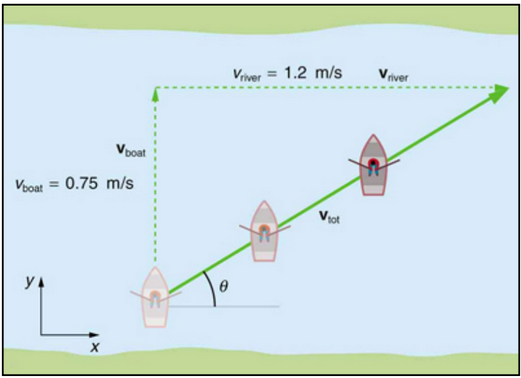
\includegraphics[clip,width = .57\columnwidth]{p1_f1}
\end{center}
\end{figure}

\eje Calcule la velocidad del viento $v_w$ para la situación que se muestra en la figura adjunta: se sabe que el avión se mueve a una velocidad $v_p$ de 45 m/s hacia el norte en relación con la masa de aire, mientras que su velocidad en relación con el suelo (su velocidad total = $v_{tot}$) es de 38 m/s en una
dirección 20° al oeste del norte.
\begin{figure}[H]
\begin{center}
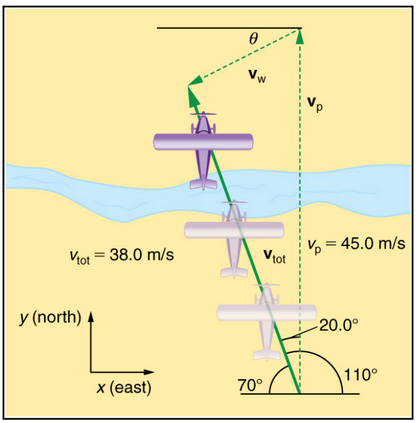
\includegraphics[clip,width = .4\columnwidth]{p1_f2}
\end{center}
\end{figure}

\eje [16] Un Lamborghini Reventón pasa con velocidad constante de 108 km/h, en ruta rectilínea,
frente al viejito de Newton (y... tiene 291 años), quien hacía las compras. Del susto, al viejito de
Newton se le caen las manzanas. Enojadísimo, se sube a su Kawasaki Ninja y, 5 s más tarde, parte con una aceleración constante de 4 m/s$^2$ hasta llegar a una velocidad de 144 km/h, que luego mantendrá constante (sino se marea... la edad, vio). ¿A qué distancia del primer encuentro se cruzarán de nuevo el Reventón y Newton en la Ninja? Trazar los gráficos correspondientes.

\eje [20] Al viejito de Newton se le escapa la manzana que tiene en la mano (sí, hay algo raro entre
las manzanas y Newton), a 80 cm sobre el piso. ¿Qué velocidad tendría la manzana al llegar al piso? ¿Cuánto tiempo tiene el viejito de Newton para evitar comer una manzana amoratada?

\eje [21] Entregado a la ciencia, el viejito de Newton se dispara verticalmente hacia arriba, con una velocidad de 30 m/s. Se pide:

a) elegir un sistema de referencia, que mantendrá invariable en todo el desarrollo, y plantear las ecuaciones del movimiento. Justificar los valores y signos asignados;

b) calcular su posición y velocidad al cabo de 2, 4 y 8 s de su lanzamiento. Hallar los desplazamientos entre 0 y 2 s; entre 2 y 4 s y entre 4 y 8 s. Interpretar;

c) determinar en qué instante el viejito de Newton vuelve a pasar por el punto de partida;

d) determinar el instante para el que su altura es máxima, y el valor de dicha altura;

e) hallar en qué instante se encuentra a 25 m de altura;

f) graficar la altura alcanzada, la velocidad y la aceleración del viejito, en función del tiempo.

Note que si el viejito se dispara verticalmente desde un sitio en la superficie de la tierra, cuando vuelve al sitio del lanzamiento, si no hubiera algún tipo de túnel que le permita atravesar hacia abajo
el nivel del suelo, se estrellaría contra el suelo. Hagamos de cuenta, por el bienestar de nuestro viejito, que al caer de vuelta entra en un túnel vertical...

\eje [27] No estando satisfecho con los resultados del experimento anterior, el viejito de Newton se coloca un cohete en la espalda y parte del reposo a nivel del piso, impulsado verticalmente hacia
arriba con una aceleración que se supone constante, mientras dura el combustible del tanque. Este se agota a los 5 s de partir, cuando el viejito de Newton está a 100 m de altura. Desde ese instante, el viejito de Newton se mueve libremente (“¡¡ahh libertad!!”), hasta que regresa al punto de partida.

a) Determinar la máxima velocidad que alcanzará al ascender;

b) a qué altura (máxima) del piso llegará;

c) trazar los gráficos de aceleración, velocidad y posición del viejito de Newton en función del tiempo, desde que parte hasta que vuelve al piso. 

Puede considerar que durante los primeros 5 s se tiene sólo la aceleración del cohete (¡aunque no sea
cierto! ¿Por qué?).


\eje [1] El viejito de Newton vuelve a la “carga” y se dispara desde lo alto de una colina con un cañón. El viejito de Newton (versión proyectil) parte con una velocidad de 50 m/s, en una dirección que
forma un ángulo de 37° con la horizontal. Elegir un sistema de referencia y, despreciando todo rozamiento:

a) hallar la posición del viejito de Newton a los 2, 5 y 8 s de haber partido, respectivamente. Representar en un diagrama su trayectoria;

b) determinar las componentes de los vectores velocidad en los instantes anteriores. Representar dichos vectores en las cuatro posiciones conocidas del diagrama anterior;

c) hallar en qué instante se encuentra al mismo nivel que el de partida, qué posición ocupa y cuál es su velocidad en ese instante;

d) sin hacer cuentas, justifique entre qué instantes de los especificados cree usted que el viejito de Newton alcanzará la máxima altura. ¿Qué velocidad tendrá allí? Calcúlelo ahora y
verifique su hipótesis;

e) con toda la información anterior, dibujar la trayectoria del viejito de Newton. Escribir la ecuación de la misma.

\eje [4] El viejito de Newton arroja horizontalmente su manzana desde la ventana de la abadía de Westminster, y la recibe a 1.2 m de altura sobre el piso, 0.8 s después (sí, Newton también sabe teletransportarse). Sabiendo que el viejito de Newton atrapa la manzana a 4.8 m del frente de la abadía, hallar:

a) a qué altura del piso partió la manzana;

b) con qué velocidad llegó a las manos del teleportado viejito de Newton;

c) cuál es la ecuación de la trayectoria de la manzana.

\eje [2.13] El viejito de Newton le lanza su Principia Mathematica de manera vertical hacia arriba a Leibniz para que lo lea, quien se asoma por una ventana unos 4 m arriba del primero, atrapando el libro 1.5 s después de haber sido lanzado.

a)¿Con qué velocidad inicial Newton arrojó su Principia?

b)¿Y con qué velocidad venía el Principia cuando fue atrapado por Leibniz?

\eje [pri.inst.prob1] Una persona arroja un ladrillo con cierto ángulo respecto del suelo (y a cierta altura del mismo), su hermano, parado a 18 m y en la dirección que arroja el ladrillo, sale
corriendo al mismo tiempo que el ladrillo abandona la mano del primero y en la dirección en la que fue arrojado, con una velocidad media de 7 m/s, y corre con esa velocidad por un intervalo de
2 s. Finalmente, atrapa el ladrillo a la misma altura a la que fue lanzado por su hermano.

a) ¿Cuál fue la velocidad ($v_0$) y el ángulo inicial $\theta_0$ con los que el primer hermano lanzó el ladrillo?

b) Encuentre la posición $(x,y)$ y velocidad ($v_x,v_y$) del ladrillo 0.1 s antes de ser atrapado por el segundo hermano.

\eje [3.7] Se lanza una pelota, con velocidad inicial 25 m/s y ángulo respecto de la horizontal de 40°, directamente hacia un muro, como se muestra en la figura que se adjunta. El muro está a 22 m
de donde se lanzó la pelota.
\begin{figure}[H]
\begin{center}
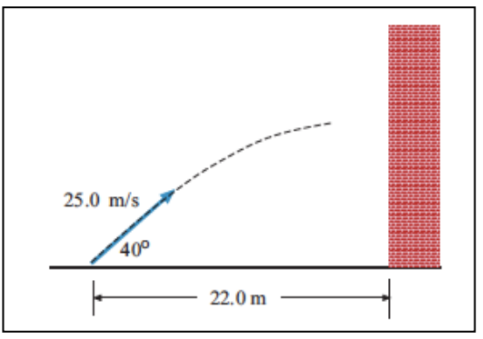
\includegraphics[clip,width = .57\columnwidth]{p1_f11}
\end{center}
\end{figure}
a) ¿Cuánto tarda la pelota en alcanzar el muro?

b) ¿A qué altura por encima del nivel dónde fue lanzada la pelota, esta última golpea al muro?
 
c) ¿Cuándo la pelota golpea el muro, lo hace antes o después de haber alcanzado su altura
máxima?

\eje [3.9 y 3.10] Un proyectil fue lanzado desde el nivel del suelo con velocidad $v_0$ y un ángulo $\theta_0$ por sobre la horizontal como muestra la figura adjunta. Encuentre:
\begin{figure}[H]
\begin{center}
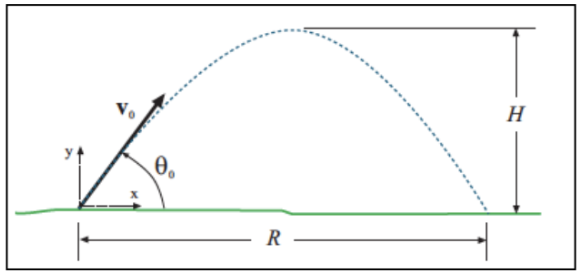
\includegraphics[clip,width = .57\columnwidth]{p1_f12}
\end{center}
\end{figure}
a) La altura máxima H a la que llega el proyectil.

b) La distancia desde el punto de partida en la que el proyectil hace impacto con el suelo, la que se denomina el rango R del proyectil.

c) Supongamos ahora que el proyectil es disparado de tal manera que su alcance horizontal R es igual al triple de la altura máxima H que logra durante su trayectoria. ¿Cuál es el ángulo con el cual fue disparado?

\eje \textcolor{blue}{[3.12] \textit{Este es difícil, si sale ya tienen cocinado Cinemática.} Un proyectil es disparado hacia arriba por un plano inclinado de ángulo $\phi$ con una velocidad inicial $v_0$ a un ángulo $\theta_0$ con respecto a la horizontal del suelo (siendo $\theta_0 > \phi$ ).}
\begin{figure}[H]
\begin{center}
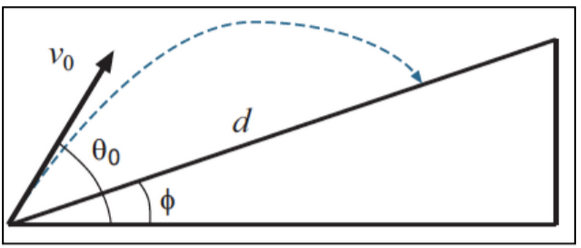
\includegraphics[clip,width = .57\columnwidth]{p1_f13}
\end{center}
\end{figure}
\textcolor{blue}{a) Muestre que el proyectil viaja una distancia d = [2 $v_0 ^2$ cos($\theta_0$) sin( $\theta_0$ - $\phi$ )]/[g cos$^2$($\phi$ )] por el plano inclinado.}

\textcolor{blue}{¿Para qué valor de $\theta_0$ es “d” un máximo, y cuál sería ese valor?}

\eje [3.13] En uno de los modelos del átomo de hidrógeno, un electrón órbita al protón en una trayectoria circular de radio $5.28\times 10^{-11}$ m con una velocidad de $2.18\times 10^6$  m/s.

a)¿Cuál es la aceleración del electrón en este modelo?

b)¿Cuál es el período de su movimiento?

\eje [3.15] Un río tiene una velocidad de 0.5 m/s. Un estudiante nada contra corriente una distancia de 1 km y vuelve al punto de partida. Si el estudiante puede nadar a una velocidad de 1.2 m/s en
agua estanca:

a) ¿cuánto puede tomarle en completar todo el trayecto?

b) Compare con el tiempo que le llevaría si nadase en agua estanca.

\end{document}